%==============================================================================
%  PRESENTACIÓN BEAMER — TALLER POISSON Y LAPLACE
%  Compilar en Overleaf con pdflatex
%  Subir junto con: ejercicio1_resultado.png ... ejercicio4_resultado.png
%==============================================================================
\documentclass[aspectratio=169, 11pt]{beamer}

%--- Tema base limpio (sin conflictos de paleta) ---
\usetheme{Boadilla}

%--- Colores personalizados ---
\definecolor{azulfc}{RGB}{15, 55, 115}
\definecolor{azulmed}{RGB}{41, 128, 185}
\definecolor{verdek}{RGB}{39, 174, 96}
\definecolor{rojok}{RGB}{192, 57, 43}
\definecolor{naranjak}{RGB}{211, 84, 0}
\definecolor{grisf}{RGB}{245, 246, 250}
\definecolor{codebg}{RGB}{248,248,248}

%--- Aplicar colores al tema ---
\setbeamercolor{structure}{fg=azulfc}
\setbeamercolor{frametitle}{bg=azulfc, fg=white}
\setbeamercolor{title}{fg=white}
\setbeamercolor{subtitle}{fg=azulmed!80!white}
\setbeamercolor{author}{fg=white}
\setbeamercolor{date}{fg=white}
\setbeamercolor{institute}{fg=white}
\setbeamercolor{footline}{bg=azulfc!90, fg=white}
\setbeamercolor{block title}{bg=azulfc, fg=white}
\setbeamercolor{block body}{bg=grisf, fg=black}
\setbeamercolor{alertblock title}{bg=rojok, fg=white}
\setbeamercolor{alertblock body}{bg=rojok!8, fg=black}
\setbeamercolor{exampleblock title}{bg=verdek!75!black, fg=white}
\setbeamercolor{exampleblock body}{bg=verdek!8, fg=black}
\setbeamercolor{titlelike}{fg=white, bg=azulfc}

%--- Fondo de portada ---
\setbeamercolor{background canvas}{bg=white}

%--- Sin botones de navegación ---
\setbeamertemplate{navigation symbols}{}

%--- Footline simple ---
\setbeamertemplate{footline}{%
  \leavevmode
  \hbox{%
    \begin{beamercolorbox}[wd=0.5\paperwidth, ht=2.4ex, dp=1ex, left, leftskip=4pt]{footline}%
      \usebeamerfont{author in head/foot}\small Modelamiento FC — Taller Poisson \& Laplace
    \end{beamercolorbox}%
    \begin{beamercolorbox}[wd=0.5\paperwidth, ht=2.4ex, dp=1ex, right, rightskip=4pt]{footline}%
      \usebeamerfont{date in head/foot}\small
      \insertframenumber\,/\,\inserttotalframenumber
    \end{beamercolorbox}%
  }%
}

%--- Encabezado con sección ---
\setbeamertemplate{headline}{%
  \leavevmode
  \begin{beamercolorbox}[wd=\paperwidth, ht=1.6ex, dp=0.5ex, center]{structure}%
    \usebeamerfont{section in head/foot}\small\insertsectionhead
  \end{beamercolorbox}%
}

%--- Paquetes ---
\usepackage[utf8]{inputenc}
\usepackage[T1]{fontenc}
\usepackage[spanish]{babel}
\usepackage{amsmath, amssymb}
\usepackage{graphicx}
\usepackage{booktabs}
\usepackage{colortbl}
\usepackage{multirow}
\usepackage{listings}
\usepackage{tikz}
\usetikzlibrary{positioning, arrows.meta}

%--- Estilo de código ---
\lstdefinestyle{mcode}{
  backgroundcolor=\color{codebg},
  frame=single, framerule=0.4pt, rulecolor=\color{gray!40},
  basicstyle=\ttfamily\scriptsize,
  keywordstyle=\color{azulfc}\bfseries,
  commentstyle=\color{verdek!70!black}\itshape,
  stringstyle=\color{rojok},
  numbers=none, breaklines=true,
  tabsize=2, showstringspaces=false,
}

%--- Metadatos ---
\title[FDM Jacobi — Poisson \& Laplace]{%
  Solución Numérica de Ecuaciones\\[0.2cm]
  de Poisson y Laplace}
\subtitle{Diferencias Finitas — Iteración de Jacobi\\
  \small Comparativa: Fortran · C++ · Python/numpy}
\author[Modelamiento FC]{Modelamiento en Física Computacional}
\date{Marzo 2026}

%==============================================================================
\begin{document}
%==============================================================================

%--- PORTADA ---
{
\setbeamercolor{background canvas}{bg=azulfc}
\setbeamercolor{normal text}{fg=white}
\begin{frame}[plain]
  \vspace{0.8cm}
  \begin{center}
    {\color{white}\Large\textbf{Modelamiento en Física Computacional}}\\[0.2cm]
    {\color{azulmed!60!white}\normalsize Taller Práctico}\\[0.6cm]
    \textcolor{white}{\rule{0.8\linewidth}{0.8pt}}\\[0.5cm]
    {\color{white}\LARGE\textbf{Solución Numérica de Ecuaciones}}\\[0.2cm]
    {\color{white}\LARGE\textbf{de Poisson y Laplace}}\\[0.2cm]
    {\color{azulmed!70!white}\normalsize Diferencias Finitas + Iteración de Jacobi}\\[0.3cm]
    \textcolor{white}{\rule{0.8\linewidth}{0.8pt}}\\[0.5cm]
    {\color{white}\normalsize\textbf{Comparativa:} Fortran · C++ · Python (numpy)}\\[0.2cm]
    {\color{white}\normalsize Mallas $100\times100$ y $500\times500$ — Doble precisión}\\[0.6cm]
    {\color{azulmed!70!white}\small Marzo 2026}
  \end{center}
\end{frame}
}

%--- ÍNDICE ---
\begin{frame}{Contenido}
  \tableofcontents
\end{frame}

%==============================================================================
\section{Problemas Físicos}
%==============================================================================

\begin{frame}{Ecuaciones de Poisson y Laplace}
  \begin{columns}[T]
    \begin{column}{0.46\textwidth}
      \begin{block}{Forma general (2D)}
        \[
          \nabla^2 V =
          \frac{\partial^2 V}{\partial x^2} +
          \frac{\partial^2 V}{\partial y^2} = f(x,y)
        \]
        \begin{itemize}
          \item $f=0$ \;\;→\; \textbf{Laplace}
          \item $f\neq0$ \;→\; \textbf{Poisson}
        \end{itemize}
      \end{block}
      \vspace{0.3cm}
      \begin{exampleblock}{Aplicaciones}
        \begin{itemize}
          \item Electrostática
          \item Conducción de calor (régimen permanente)
          \item Flujo potencial
          \item Mecánica estructural
        \end{itemize}
      \end{exampleblock}
    \end{column}
    \begin{column}{0.50\textwidth}
      \begin{alertblock}{Objetivo del taller}
        Resolver \textbf{4 EDPs} con solución analítica conocida
        en tres lenguajes y comparar rendimiento.
      \end{alertblock}
      \vspace{0.3cm}
      \begin{block}{Lenguajes comparados}
        \begin{tabular}{ll}
          \toprule
          \textbf{Lenguaje} & \textbf{Estrategia} \\
          \midrule
          Fortran & Bucles DO, arrays contig. \\
          C++     & \texttt{vector<vector<double>>} \\
          Python  & numpy vectorizado \\
          \bottomrule
        \end{tabular}
      \end{block}
    \end{column}
  \end{columns}
\end{frame}

\begin{frame}{Los Cuatro Problemas}
  \small
  \begin{columns}[T]
    \begin{column}{0.48\textwidth}
      \begin{block}{E1 — Poisson exponencial}
        $\nabla^2 V = (x^2+y^2)e^{xy},\quad [0,2]\times[0,1]$\\[0.15cm]
        CC: $V(0,y)=1$,\; $V(2,y)=e^{2y}$,\; $V(x,0)=1$,\; $V(x,1)=e^x$\\[0.15cm]
        \textbf{Analítica:} $V = e^{xy}$
      \end{block}
      \vspace{0.2cm}
      \begin{block}{E2 — Laplace}
        $\nabla^2 V = 0,\quad [1,2]\times[0,1]$\\[0.15cm]
        CC: $V(1,y)=\ln(y^2+1)$,\; $V(2,y)=\ln(y^2+4)$,\\
        \hphantom{CC: }$V(x,0)=2\ln x$,\; $V(x,1)=\ln(x^2+1)$\\[0.15cm]
        \textbf{Analítica:} $V = \ln(x^2+y^2)$
      \end{block}
    \end{column}
    \begin{column}{0.48\textwidth}
      \begin{block}{E3 — Poisson fuente constante}
        $\nabla^2 V = 4,\quad [1,2]\times[0,2]$\\[0.15cm]
        CC: consistentes con $(x-y)^2$\\[0.15cm]
        \textbf{Analítica:} $V = (x-y)^2$
      \end{block}
      \vspace{0.2cm}
      \begin{block}{E4 — Poisson fuente variable}
        $\nabla^2 V = \tfrac{x}{y}+\tfrac{y}{x},\quad [1,2]\times[1,2]$\\[0.15cm]
        CC: $V(1,y)=y\ln y$,\; $V(2,y)=2y\ln(2y)$,\\
        \hphantom{CC: }$V(x,1)=x\ln x$,\; $V(x,2)=2x\ln(2x)$\\[0.15cm]
        \textbf{Analítica:} $V = xy\ln(xy)$
      \end{block}
    \end{column}
  \end{columns}
\end{frame}

%==============================================================================
\section{Método Numérico}
%==============================================================================

\begin{frame}{Discretización — Esquema de 5 Puntos}
  \begin{columns}[T]
    \begin{column}{0.55\textwidth}
      Malla uniforme: $h=\Delta x$, $k=\Delta y$\\[0.2cm]
      Diferencias centradas de orden 2:
      \[
        \frac{\partial^2 V}{\partial x^2} \approx \frac{V_{i,j+1}-2V_{i,j}+V_{i,j-1}}{h^2}
      \]
      \[
        \frac{\partial^2 V}{\partial y^2} \approx \frac{V_{i+1,j}-2V_{i,j}+V_{i-1,j}}{k^2}
      \]
      \vspace{0.2cm}
      \textbf{Ecuación de actualización:}
      \[
        \boxed{
          V_{i,j} = \frac{(V_{i+1,j}+V_{i-1,j})k^2+(V_{i,j+1}+V_{i,j-1})h^2-f_{i,j}h^2k^2}{2(h^2+k^2)}
        }
      \]
      \vspace{0.1cm}
      {\small Error de discretización: $\mathcal{O}(h^2+k^2)$ — \textbf{orden 2}}
    \end{column}
    \begin{column}{0.40\textwidth}
      \begin{center}
      \begin{tikzpicture}[scale=1.15]
        \draw[gray!30] (0,0) grid (2,2);
        \fill[azulfc] (0,1) circle (3.5pt);
        \fill[azulfc] (2,1) circle (3.5pt);
        \fill[azulfc] (1,0) circle (3.5pt);
        \fill[azulfc] (1,2) circle (3.5pt);
        \fill[rojok]  (1,1) circle (4pt);
        \node[left,  font=\small, azulfc] at (0,1)   {$V_{i,j-1}$};
        \node[right, font=\small, azulfc] at (2,1)   {$V_{i,j+1}$};
        \node[below, font=\small, azulfc] at (1,0)   {$V_{i-1,j}$};
        \node[above, font=\small, azulfc] at (1,2)   {$V_{i+1,j}$};
        \node[above right, font=\small\bfseries, rojok] at (1,1) {$V_{i,j}$};
        \draw[->, azulmed, thick] (0.18,1)--(0.82,1);
        \draw[->, azulmed, thick] (1.82,1)--(1.18,1);
        \draw[->, azulmed, thick] (1,0.18)--(1,0.82);
        \draw[->, azulmed, thick] (1,1.82)--(1,1.18);
        \draw[<->, gray] (0,-0.25)--(1,-0.25) node[midway,below,font=\scriptsize]{$h$};
        \draw[<->, gray] (-0.3,0)--(-0.3,1) node[midway,left,font=\scriptsize]{$k$};
      \end{tikzpicture}
      \end{center}
    \end{column}
  \end{columns}
\end{frame}

\begin{frame}{Iteración de Jacobi}
  \begin{columns}[T]
    \begin{column}{0.52\textwidth}
      \begin{block}{Algoritmo iterativo}
        \begin{enumerate}
          \item Inicializar: $V^{(0)}=0$ en interior, CC en bordes
          \item Calcular $V^{(n+1)}$ \textbf{completo} con valores de $V^{(n)}$
          \item Medir convergencia:
          \[
            \delta = \max_{i,j}\left|V_{i,j}^{(n+1)} - V_{i,j}^{(n)}\right|
          \]
          \item Si $\delta < 10^{-6}$ → \textcolor{verdek}{\textbf{convergió}}
          \item Si $n=400\,000$ → \textcolor{rojok}{\textbf{detener}}
        \end{enumerate}
      \end{block}
      \vspace{0.2cm}
      \begin{exampleblock}{Parámetros}
        Tolerancia: $10^{-6}$ \quad Iter. máx.: $400\,000$ \quad Precisión: 64-bit
      \end{exampleblock}
    \end{column}
    \begin{column}{0.44\textwidth}
      \begin{alertblock}{Complejidad — $\mathcal{O}(N^4)$}
        \begin{tabular}{ll}
          Trabajo/iter:   & $\mathcal{O}(N^2)$ \\[0.2cm]
          Iters. totales: & $\mathcal{O}(N^2)$ \\[0.1cm]
          \multicolumn{2}{l}{\small $\rho \approx 1-\frac{\pi^2}{2}h^2$\quad con $h=1/N$} \\[0.2cm]
          \textbf{Total:} & $\boldsymbol{\mathcal{O}(N^4)}$ \\
        \end{tabular}
      \end{alertblock}
      \vspace{0.3cm}
      \begin{block}{Característica de Jacobi}
        Requiere \textbf{2 arreglos} en memoria simultáneos ($V$ y $V_\text{new}$).\\[0.15cm]
        Fácilmente paralelizable.
      \end{block}
    \end{column}
  \end{columns}
\end{frame}

%==============================================================================
\section{Implementaciones}
%==============================================================================

\begin{frame}[fragile]{Fortran — \texttt{gfortran -O2}}
  \begin{columns}[T]
    \begin{column}{0.40\textwidth}
      \begin{exampleblock}{Características}
        \begin{itemize}
          \item Arrays \texttt{allocatable real(8)}
          \item Storage: \textbf{column-major}
          \item Índice $i$→$y$,\; $j$→$x$
          \item Timer: \texttt{cpu\_time()}
        \end{itemize}
      \end{exampleblock}
      \vspace{0.2cm}
      \begin{block}{Por qué es el más rápido}
        Arrays \textbf{contiguos} + bucles DO → máxima localidad de caché.\\
        \texttt{-O2} vectoriza el inner loop.
      \end{block}
    \end{column}
    \begin{column}{0.57\textwidth}
\begin{lstlisting}[style=mcode, language=Fortran,
  morekeywords={do,end,if,then,exit,real,max,abs,write}]
do it = 1, 400000
  delta = 0.0d0
  do i = 1, N-1
    do j = 1, M-1
      T_new(i,j) = (                     &
          (T(i+1,j)+T(i-1,j))*k2         &
        + (T(i,j+1)+T(i,j-1))*h2         &
        - source(i,j)*h2*k2              &
        ) / denom
      delta = max(delta,                  &
              abs(T_new(i,j)-T(i,j)))
    end do
  end do
  T = T_new
  if (delta < tol) exit
end do
\end{lstlisting}
    \end{column}
  \end{columns}
\end{frame}

\begin{frame}[fragile]{C++ — \texttt{g++ -O2}}
  \begin{columns}[T]
    \begin{column}{0.40\textwidth}
      \begin{block}{Características}
        \begin{itemize}
          \item \texttt{vector<vector<double>>}
          \item Storage: \textbf{heap no contiguo}
          \item Timer: \texttt{chrono}
          \item Fuente via \texttt{switch}
        \end{itemize}
      \end{block}
      \vspace{0.2cm}
      \begin{alertblock}{Limitación}
        Acceso a \texttt{V[i$\pm$1][j]} sigue punteros no contiguos → \textbf{cache misses} en dirección $y$.
      \end{alertblock}
    \end{column}
    \begin{column}{0.57\textwidth}
\begin{lstlisting}[style=mcode, language=C++]
while (delta > TOLERANCE
       && iters < MAX_ITERATIONS) {
    delta = 0.0;
    V_old = V;
    for (int i = 1; i < M; ++i) {
      for (int j = 1; j < N; ++j) {
        double f = source_term(
                     x_ini+i*h,
                     y_ini+j*k);
        V[i][j] = (
          (V_old[i+1][j]+V_old[i-1][j])*(k*k)
         +(V_old[i][j+1]+V_old[i][j-1])*(h*h)
         - f*h2k2) / denom;
        delta = std::max(delta,
          std::abs(V[i][j]-V_old[i][j]));
      }
    }
    iters++;
}
\end{lstlisting}
    \end{column}
  \end{columns}
\end{frame}

\begin{frame}[fragile]{Python/numpy}
  \begin{columns}[T]
    \begin{column}{0.40\textwidth}
      \begin{block}{Características}
        \begin{itemize}
          \item Arrays numpy: \textbf{contiguos} (C row-major)
          \item \textbf{Sin bucles} Python en el inner loop
          \item Jacobi 100\% vectorizado
          \item Timer: \texttt{perf\_counter()}
        \end{itemize}
      \end{block}
      \vspace{0.2cm}
      \begin{exampleblock}{Por qué es competitivo}
        Slices de numpy ejecutan en \textbf{C nativo}.\\
        Memoria contigua → sin cache misses.
      \end{exampleblock}
    \end{column}
    \begin{column}{0.57\textwidth}
\begin{lstlisting}[style=mcode, language=Python]
for it in range(1, MAX_ITER + 1):
    T_new = T.copy()

    T_new[1:-1, 1:-1] = (
        (T[2:,   1:-1] + T[:-2, 1:-1]) * k2
      + (T[1:-1, 2:]   + T[1:-1, :-2]) * h2
      - source[1:-1, 1:-1] * h2 * k2
    ) / denom

    delta = np.max(
        np.abs(T_new[1:-1,1:-1]
               - T[1:-1,1:-1]))
    T = T_new
    if delta < TOL:
        break
\end{lstlisting}
    \end{column}
  \end{columns}
\end{frame}

%==============================================================================
\section{Resultados — Soluciones}
%==============================================================================

\begin{frame}{E1 — Poisson: $\nabla^2V=(x^2+y^2)e^{xy}$\quad$\Rightarrow$\quad$V=e^{xy}$}
  \begin{center}
    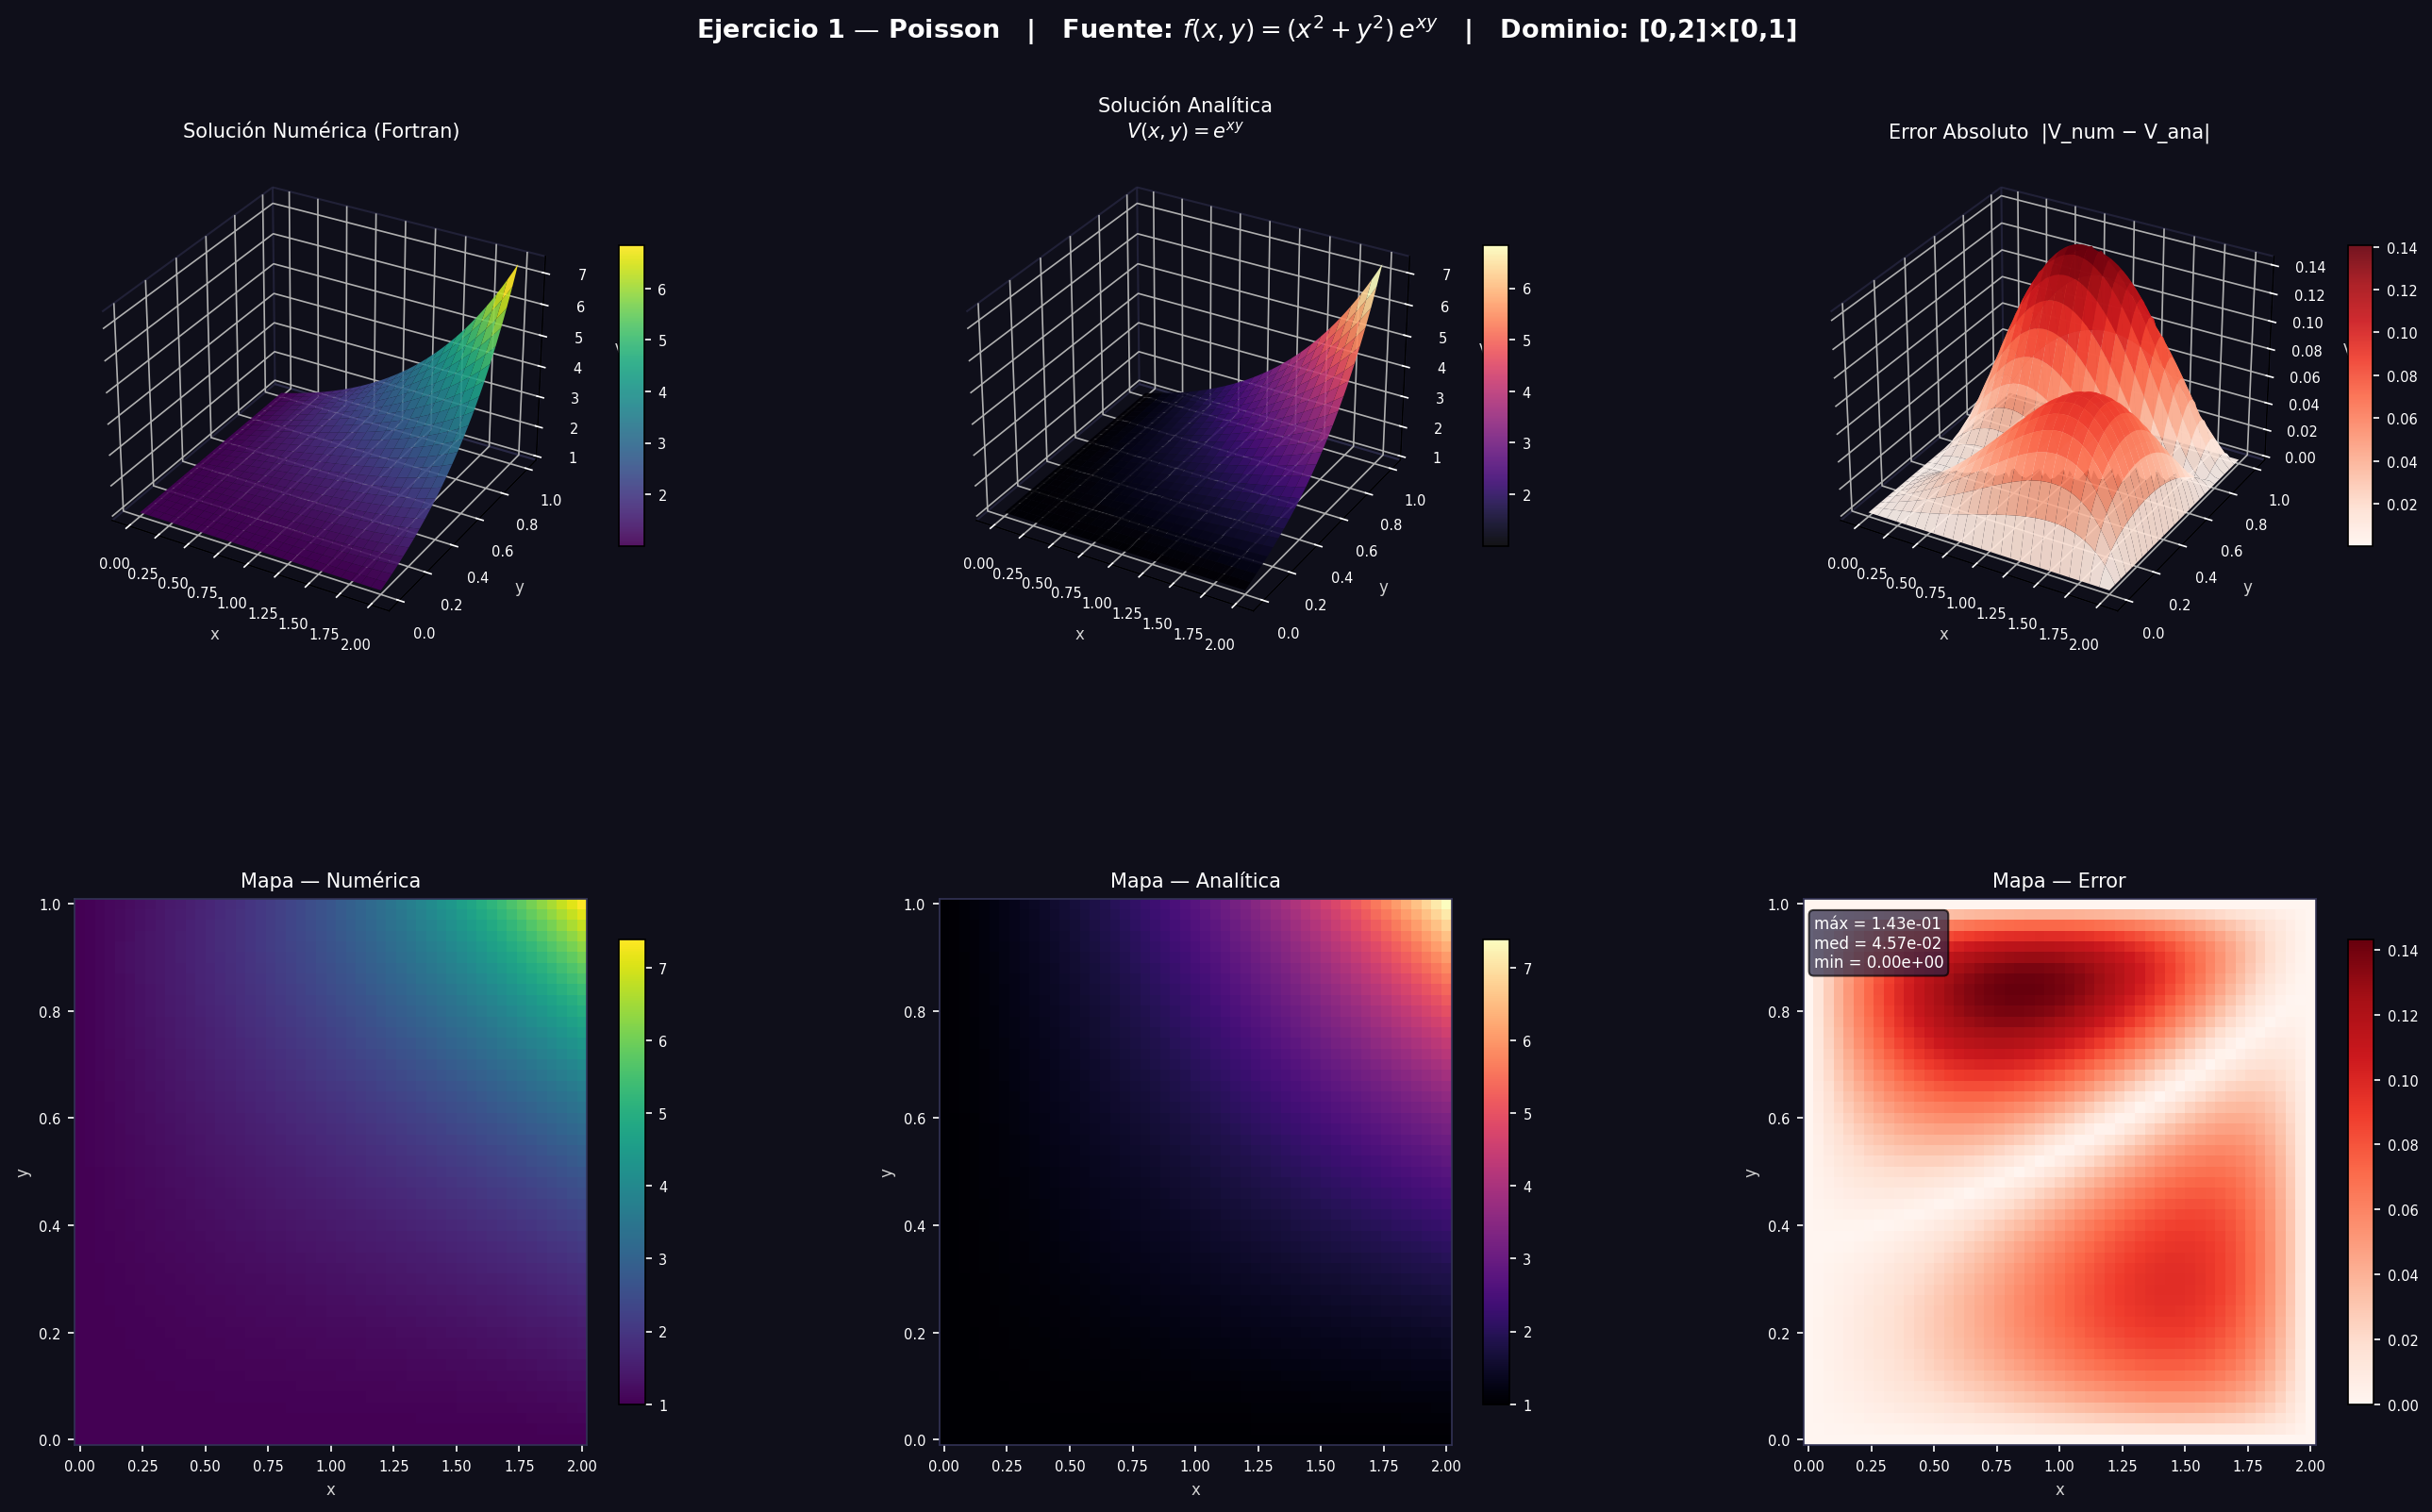
\includegraphics[width=0.90\textwidth]{ejercicio1_resultado.png}
  \end{center}
  \vspace{-0.2cm}
  {\centering\small Malla $100\times100$ · \textbf{14\,672 iteraciones} · Error máx. $1.4\times10^{-1}$ (gradiente alto en $x=2,y=1$)\par}
\end{frame}

\begin{frame}{E2 — Laplace: $\nabla^2V=0$\quad$\Rightarrow$\quad$V=\ln(x^2+y^2)$}
  \begin{center}
    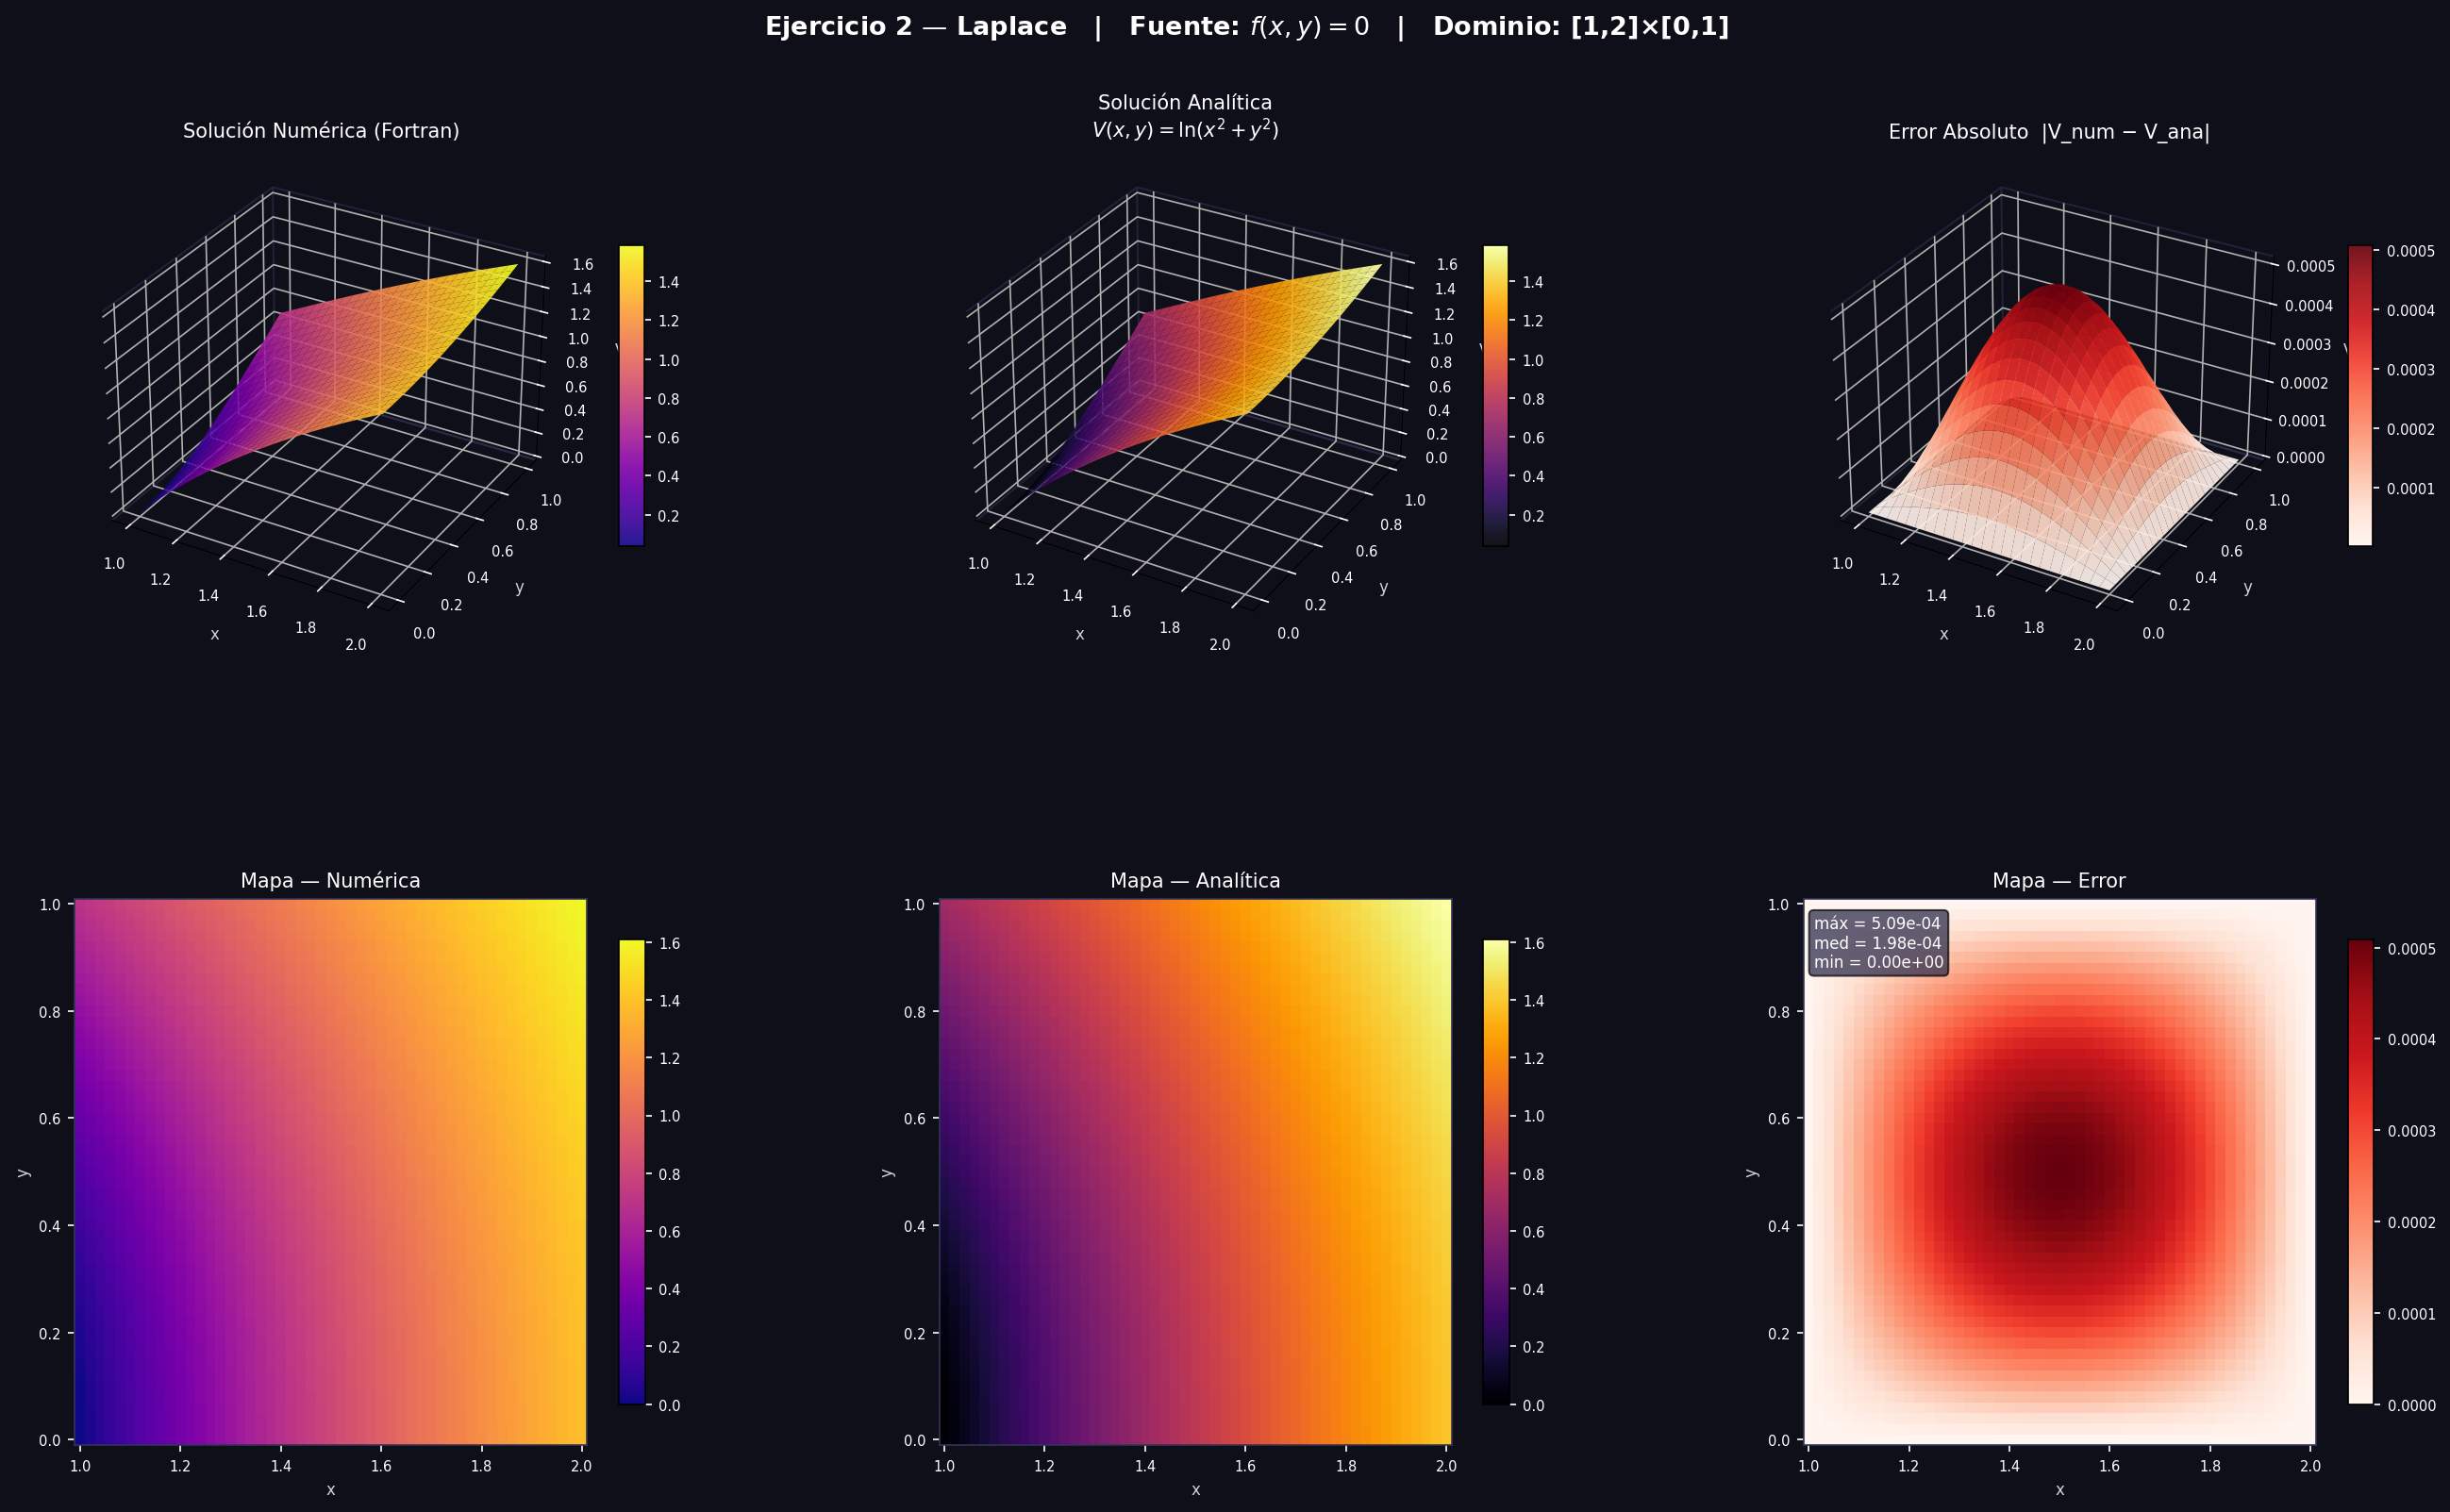
\includegraphics[width=0.90\textwidth]{ejercicio2_resultado.png}
  \end{center}
  \vspace{-0.2cm}
  {\centering\small Malla $100\times100$ · \textbf{13\,368 iteraciones} · Error máx. $2.0\times10^{-3}$ (solución suave, sin fuente interna)\par}
\end{frame}

\begin{frame}{E3 — Poisson: $\nabla^2V=4$\quad$\Rightarrow$\quad$V=(x-y)^2$}
  \begin{center}
    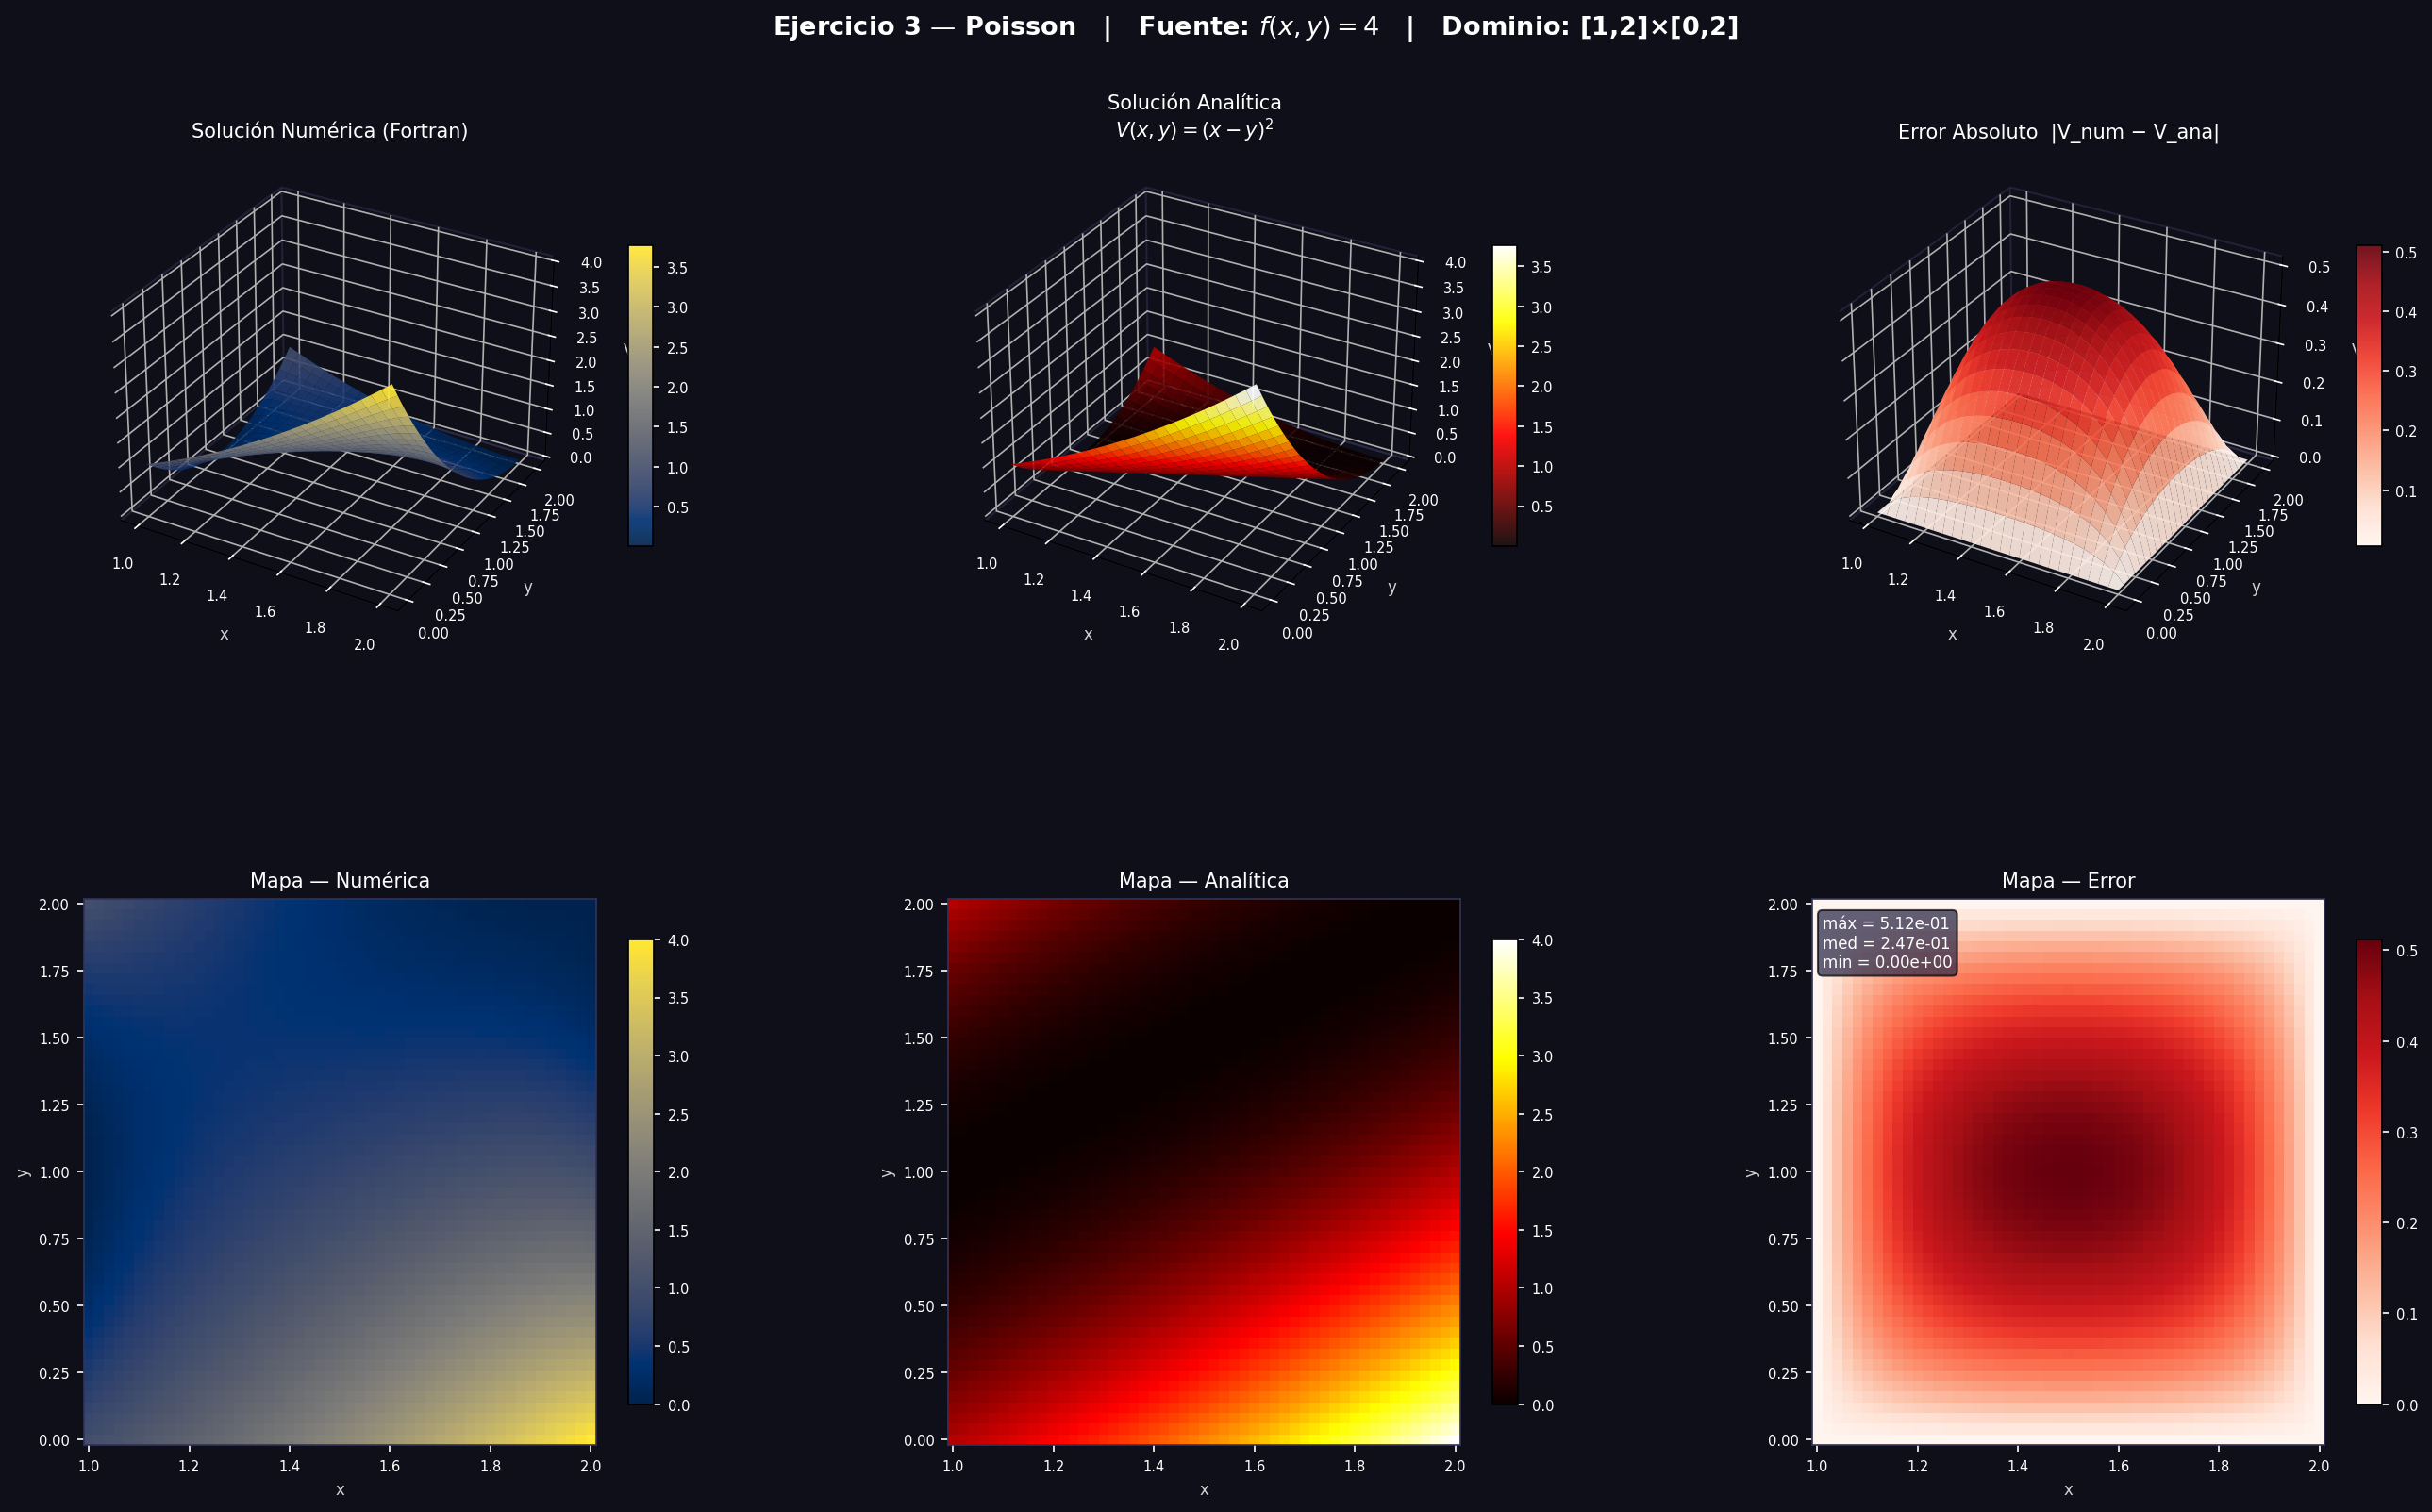
\includegraphics[width=0.90\textwidth]{ejercicio3_resultado.png}
  \end{center}
  \vspace{-0.2cm}
  {\centering\small Malla $100\times100$ · \textbf{13\,220 iteraciones} · Error máx. $5.1\times10^{-1}$ (dominio no cuadrado, gradientes en esquinas)\par}
\end{frame}

\begin{frame}{E4 — Poisson: $\nabla^2V=x/y+y/x$\quad$\Rightarrow$\quad$V=xy\ln(xy)$}
  \begin{center}
    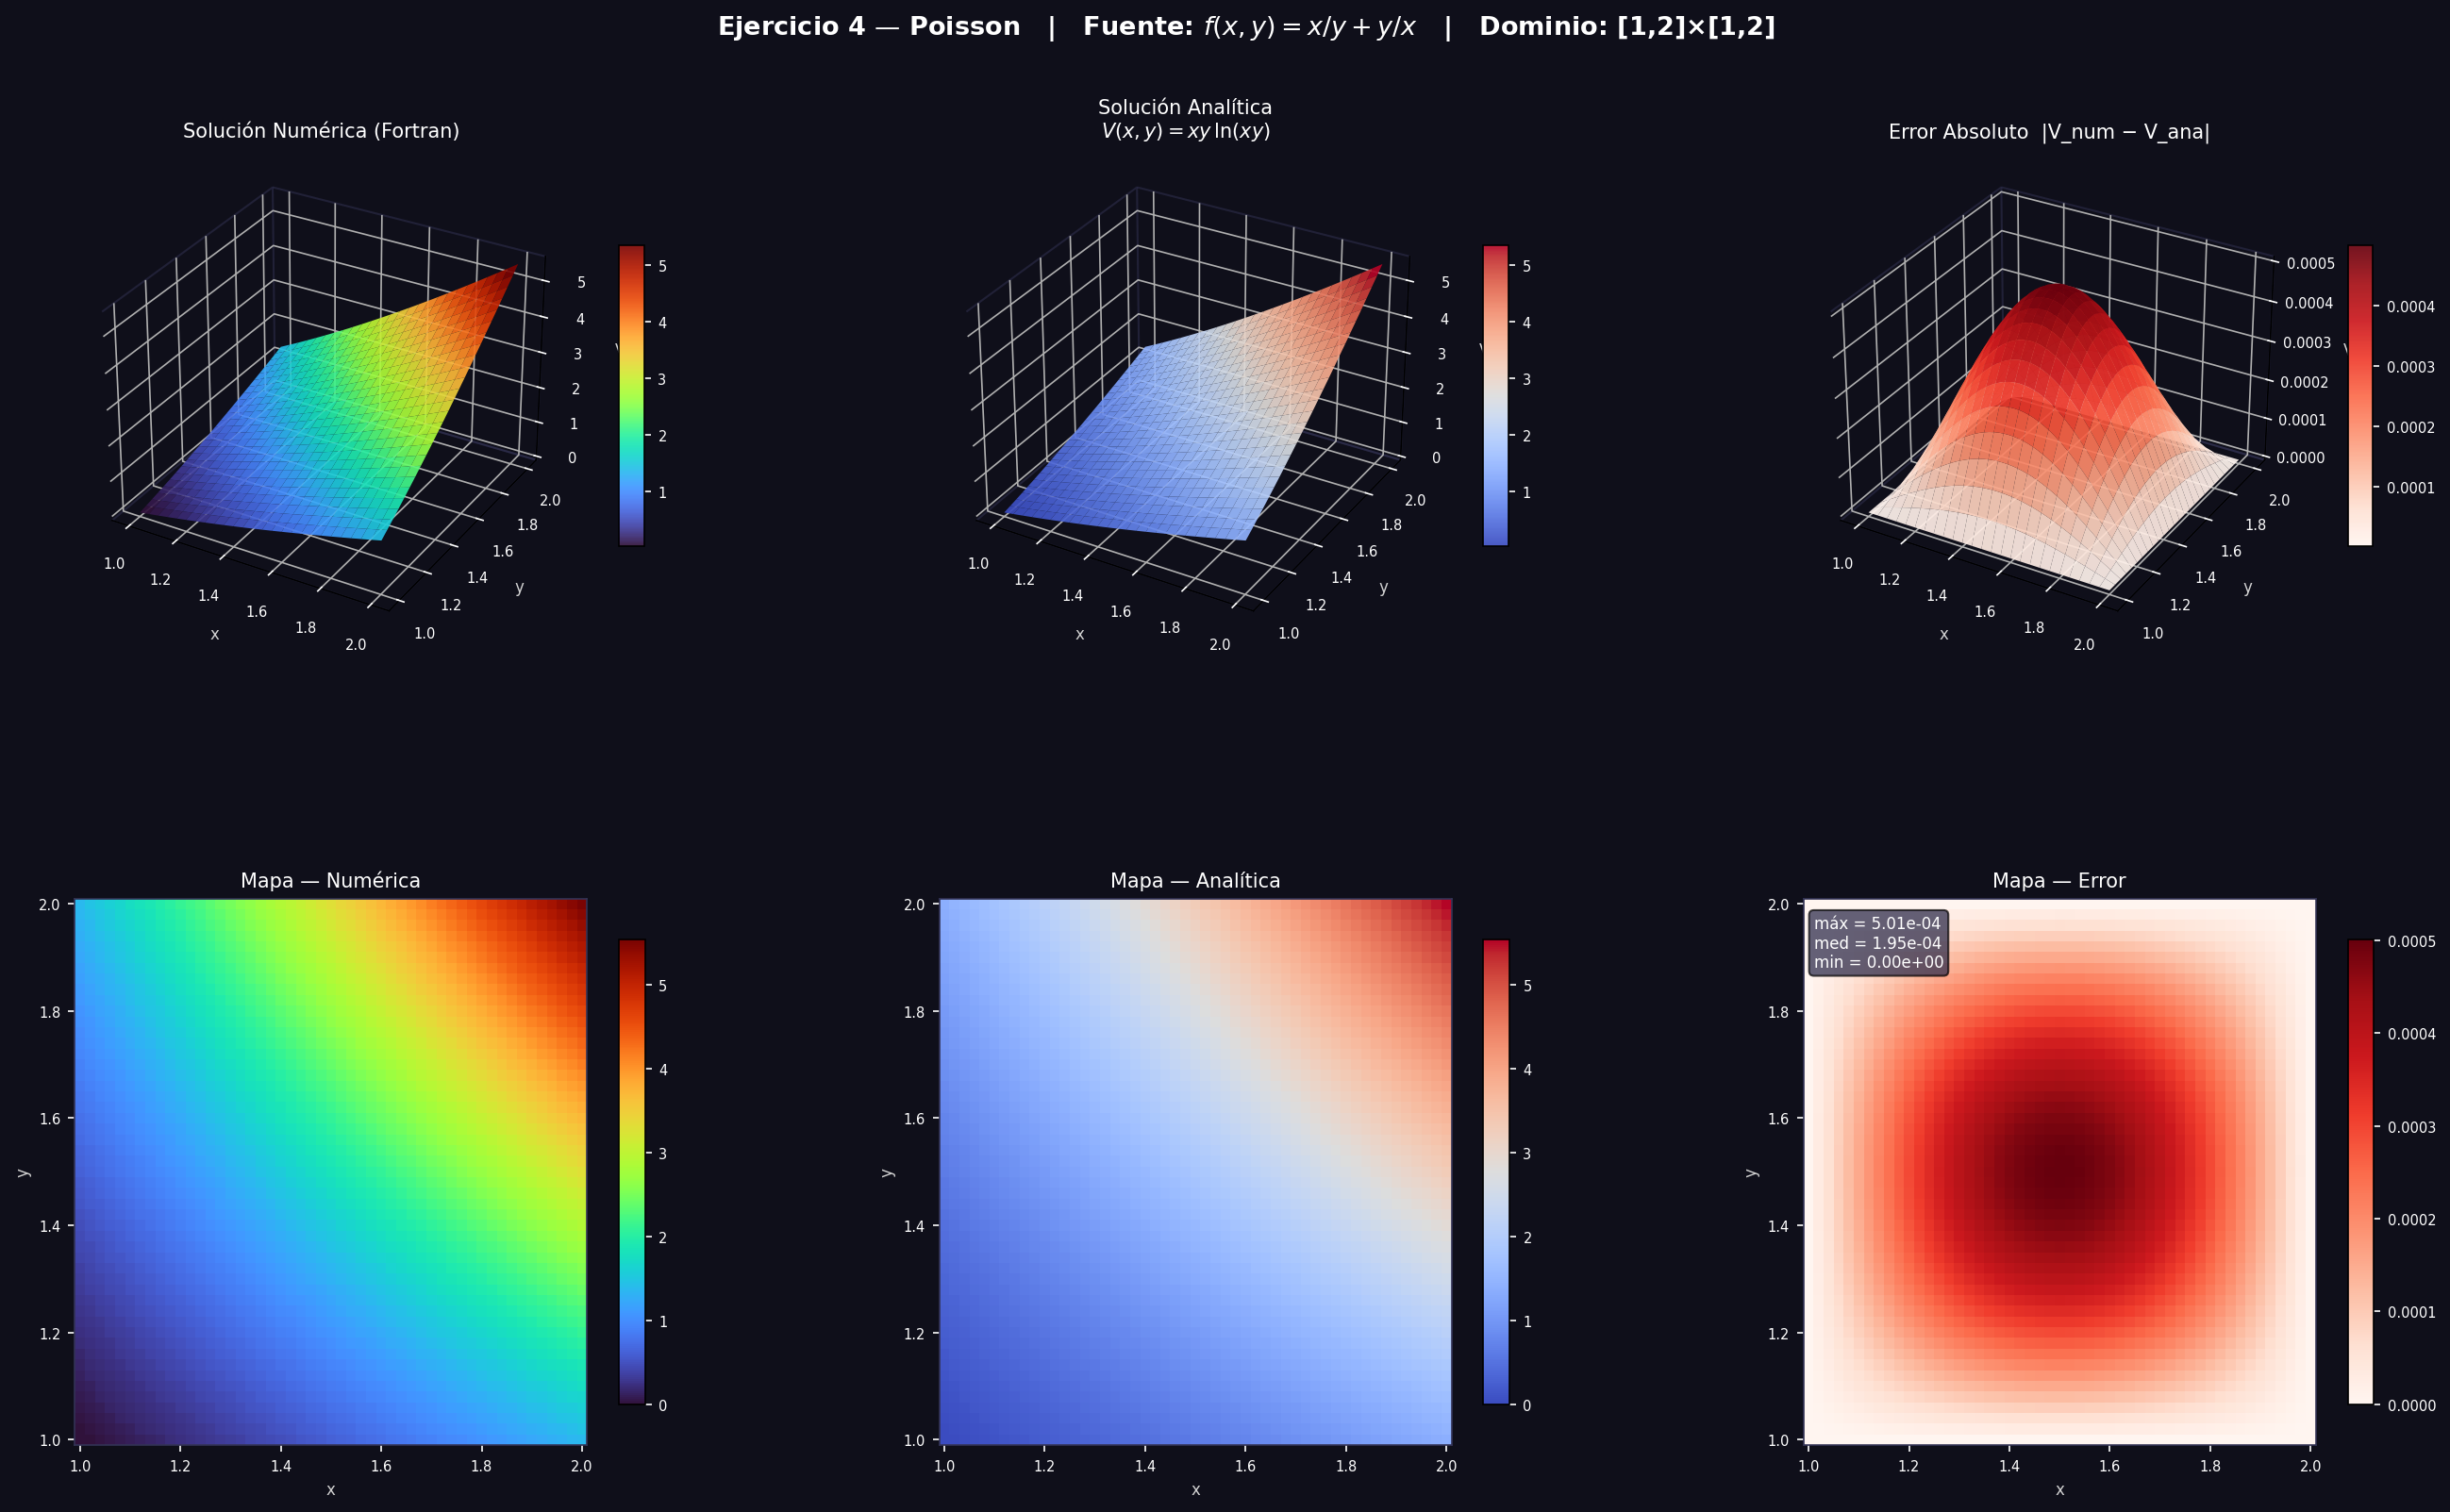
\includegraphics[width=0.90\textwidth]{ejercicio4_resultado.png}
  \end{center}
  \vspace{-0.2cm}
  {\centering\small Malla $100\times100$ · \textbf{14\,816 iteraciones} · Error máx. $2.0\times10^{-3}$ (solución suave en $[1,2]^2$)\par}
\end{frame}

%==============================================================================
\section{Benchmark}
%==============================================================================

\begin{frame}{Benchmark — Malla $100\times100$}
  \begin{columns}[T]
    \begin{column}{0.55\textwidth}
      \begin{center}
      \begin{tabular}{lccc}
        \toprule
        \textbf{Ejercicio} & \textbf{Fortran} & \textbf{C++} & \textbf{Python} \\
        \midrule
        E1 — Poisson $e^{xy}$ & 0.249 s & 0.979 s & 1.418 s \\
        E2 — Laplace          & 0.185 s & 0.361 s & 1.292 s \\
        E3 — Poisson $f=4$    & 0.220 s & 0.332 s & 1.282 s \\
        E4 — Poisson var.     & 0.245 s & 0.410 s & 1.431 s \\
        \midrule
        \rowcolor{azulfc!12}
        \textbf{Total} & \textbf{0.90 s} & \textbf{2.08 s} & \textbf{5.42 s} \\
        \bottomrule
      \end{tabular}
      \end{center}
    \end{column}
    \begin{column}{0.42\textwidth}
      \begin{block}{Speedup vs.\ Fortran}
        \begin{tabular}{lc}
          \toprule
          & Más lento \\
          \midrule
          C++    & $2.3\times$ \\
          Python & $6.0\times$ \\
          \bottomrule
        \end{tabular}
      \end{block}
      \vspace{0.3cm}
      \begin{exampleblock}{Convergencia}
        \textbf{Todos convergieron.}\\
        Las $\sim$13\,000–15\,000 iter.\\ necesarias están muy por debajo del límite de 400\,000.
      \end{exampleblock}
    \end{column}
  \end{columns}
\end{frame}

\begin{frame}{Benchmark — Malla $500\times500$}
  \begin{columns}[T]
    \begin{column}{0.60\textwidth}
      \begin{center}
      \small
      \begin{tabular}{lcccc}
        \toprule
        \textbf{Ejerc.} & \textbf{Fortran} & \textbf{C++} & \textbf{Python} & \textbf{Iter.} \\
        \midrule
        E1 & 128.96 s & 343.72 s & \cellcolor{verdek!20}301.40 s & 203\,879 \\
        E2 &  67.70 s & 122.00 s & 299.44 s & 171\,155 \\
        E3 & 103.93 s & \cellcolor{verdek!20}102.71 s & 308.36 s & 167\,653 \\
        E4 & 130.79 s & 146.96 s & 401.51 s & 207\,350 \\
        \midrule
        \rowcolor{azulfc!12}
        \textbf{Total} & \textbf{431 s} & \textbf{715 s} & \textbf{1311 s} & — \\
        \bottomrule
      \end{tabular}
      \end{center}
      \vspace{0.2cm}
      {\small\color{verdek!70!black} Las celdas verdes señalan resultados sorpresivos.}
    \end{column}
    \begin{column}{0.36\textwidth}
      \begin{alertblock}{¡Sorpresas!}
        \textbf{E1:} Python (301 s) supera a C++ (344 s)\\[0.2cm]
        \textbf{E3:} C++ (102 s) iguala a Fortran (104 s)
      \end{alertblock}
      \vspace{0.2cm}
      \begin{block}{Speedup vs.\ Fortran}
        \begin{tabular}{lc}
          \toprule
          C++    & $1.66\times$ \\
          Python & $3.04\times$ \\
          \bottomrule
        \end{tabular}
      \end{block}
    \end{column}
  \end{columns}
\end{frame}

%==============================================================================
\section{Análisis}
%==============================================================================

\begin{frame}{¿Por qué Fortran gana? — Caché y Memoria}
  \begin{columns}[T]
    \begin{column}{0.31\textwidth}
      \begin{exampleblock}{\centering Fortran}
        \centering\vspace{0.1cm}
        Array \textbf{contiguo}\\column-major\\[0.2cm]
        Bucles DO:\\acceso óptimo\\a caché L1/L2\\[0.2cm]
        \texttt{-O2} vectoriza\\inner loop\\[0.2cm]
        \textcolor{verdek}{\textbf{Caché: óptimo}}
      \end{exampleblock}
    \end{column}
    \begin{column}{0.31\textwidth}
      \begin{alertblock}{\centering C++}
        \centering\vspace{0.1cm}
        \texttt{vector<vector>}\\heap fragmentado\\[0.2cm]
        Acceso a filas\\adyacentes:\\punteros dispersos\\[0.2cm]
        \textcolor{rojok}{\textbf{Cache misses}}\\en dir.\ $y$
      \end{alertblock}
    \end{column}
    \begin{column}{0.31\textwidth}
      \begin{block}{\centering Python/numpy}
        \centering\vspace{0.1cm}
        Array numpy\\C row-major\\[0.2cm]
        Slices ejecutan\\en C nativo\\SIMD en bloques\\[0.2cm]
        \textcolor{azulmed}{\textbf{Caché: bueno}}
      \end{block}
    \end{column}
  \end{columns}
  \vspace{0.4cm}
  \begin{center}
  \begin{tikzpicture}
    \node[draw=verdek,fill=verdek!12,rounded corners,minimum width=2.8cm,
          minimum height=0.65cm,font=\small\bfseries] (f) {Fortran: 0.90 s};
    \node[draw=rojok,fill=rojok!12,rounded corners,minimum width=2.8cm,
          minimum height=0.65cm,font=\small\bfseries, right=1.2cm of f] (c) {C++: 2.08 s};
    \node[draw=naranjak,fill=naranjak!12,rounded corners,minimum width=2.8cm,
          minimum height=0.65cm,font=\small\bfseries, right=1.2cm of c] (p) {Python: 5.42 s};
    \draw[->,thick,gray] (f.east)--(c.west) node[midway,above,font=\scriptsize]{$\times$2.3};
    \draw[->,thick,gray] (c.east)--(p.west) node[midway,above,font=\scriptsize]{$\times$2.6};
    \node[below=0.15cm of c,font=\scriptsize\itshape,gray] {Malla $100\times100$ — total 4 ejercicios};
  \end{tikzpicture}
  \end{center}
\end{frame}

\begin{frame}{Python supera a C++ a $500\times500$ — ¿Por qué?}
  \begin{columns}[T]
    \begin{column}{0.48\textwidth}
      \begin{alertblock}{El cuello de botella de C++}
        \texttt{vector<vector<double>>} con $N=500$:
        \begin{itemize}
          \item 500 filas = 500 punteros independientes
          \item Cada fila $\approx$ 4 KB en posición aleatoria de memoria
          \item Acceso a \texttt{V[i+1][j]}: probable \textbf{cache miss L2}
          \item Penalización \textbf{crece con $N$}
        \end{itemize}
      \end{alertblock}
    \end{column}
    \begin{column}{0.48\textwidth}
      \begin{exampleblock}{La ventaja de numpy}
        Array contiguo en memoria:
        \begin{itemize}
          \item \texttt{T[2:,1:-1]}: acceso secuencial por filas
          \item Operaciones \textbf{SIMD} sobre bloques contiguos
          \item A $500\times500$: cuello de botella = ancho de banda de memoria, no overhead de Python
        \end{itemize}
      \end{exampleblock}
    \end{column}
  \end{columns}
  \vspace{0.3cm}
  \begin{center}
  \begin{block}{}
    \centering
    E1 — $500\times500$: \quad
    Fortran \textbf{128.96 s} \quad
    C++ \textcolor{rojok}{\textbf{343.72 s}} \quad
    Python \textcolor{verdek}{\textbf{301.40 s}}\\[0.1cm]
    {\small Python es \textbf{12\% más rápido} que C++ gracias a la contigüidad de memoria}
  \end{block}
  \end{center}
\end{frame}

\begin{frame}{Escalado $\mathcal{O}(N^4)$ y Convergencia}
  \begin{columns}[T]
    \begin{column}{0.48\textwidth}
      \begin{block}{Razón de tiempo: $100\to500$}
        \begin{tabular}{lcc}
          \toprule
          & \textbf{Obs.} & \textbf{Teórico} \\
          \midrule
          Fortran & $481\times$ & \multirow{3}{*}{$347\times$} \\
          C++     & $344\times$ & \\
          Python  & $242\times$ & \\
          \bottomrule
          \multicolumn{3}{l}{\small Iter.: $203\,879/14\,672 = 13.9\times$} \\
          \multicolumn{3}{l}{\small Trabajo/iter.: $\times25$ → $13.9\times25=347\times$} \\
        \end{tabular}
      \end{block}
    \end{column}
    \begin{column}{0.48\textwidth}
      \begin{alertblock}{Con 100\,000 iter. → no convergía}
        Error residual $\approx 0.1$–$0.5$ a $500\times500$.
      \end{alertblock}
      \vspace{0.2cm}
      \begin{exampleblock}{Con 400\,000 iter. → convergió ✓}
        \begin{tabular}{lc}
          E1 & 203\,879 \\
          E2 & 171\,155 \\
          E3 & 167\,653 \\
          E4 & 207\,350 \\
        \end{tabular}\\[0.1cm]
        Margen disponible: $\sim48\%$
      \end{exampleblock}
      \vspace{0.15cm}
      {\small Para $N\geq1000$: usar \textbf{SOR} o \textbf{Multigrid}.}
    \end{column}
  \end{columns}
\end{frame}

%==============================================================================
\section{Conclusiones}
%==============================================================================

\begin{frame}{Conclusiones}
  \begin{enumerate}
    \setlength\itemsep{0.3cm}
    \item \textbf{Fortran es el más rápido} en casi todos los casos:
          $1.7$–$2.3\times$ sobre C++ y $3$–$6\times$ sobre Python.
          Debe su rendimiento al almacenamiento contiguo y a \texttt{gfortran -O2}.

    \item \textbf{C++ no supera a Fortran} con \texttt{vector<vector<double>>}.
          El layout fragmentado genera cache misses en dirección $y$.
          La solución: usar un arreglo plano 1D con indexación manual.

    \item \textbf{Python/numpy supera a C++} en mallas grandes
          (E1, $500\times500$: 301 s vs 344 s) por acceso a memoria contiguo.

    \item \textbf{Con 400\,000 iteraciones Jacobi converge} a $500\times500$.
          Para mallas mayores se recomiendan SOR o multigrid.

    \item \textbf{Los tres códigos son algorítmicamente equivalentes}:
          mismas iteraciones, mismos errores — las diferencias son solo de rendimiento.
  \end{enumerate}
\end{frame}

%--- DIAPOSITIVA FINAL ---
{
\setbeamercolor{background canvas}{bg=azulfc}
\begin{frame}[plain]
  \begin{center}
    \vspace{1.2cm}
    \textcolor{white}{\rule{0.6\linewidth}{0.8pt}}\\[0.6cm]
    {\color{white}\LARGE\textbf{¿Preguntas?}}\\[0.8cm]
    \textcolor{white}{\rule{0.6\linewidth}{0.8pt}}\\[0.8cm]
    \begin{tabular}{ll}
      \color{white}\textbf{Fortran:} & \color{azulmed!80!white}\texttt{poisson\_laplace.f90} \\[0.2cm]
      \color{white}\textbf{C++:}     & \color{azulmed!80!white}\texttt{poisson\_serial.cpp} \\[0.2cm]
      \color{white}\textbf{Python:}  & \color{azulmed!80!white}\texttt{poisson\_serial.py} \\[0.2cm]
      \color{white}\textbf{Tolera.:} & \color{azulmed!80!white}$\delta < 10^{-6}$ \\[0.2cm]
      \color{white}\textbf{Iter.\ máx.:} & \color{azulmed!80!white}$400\,000$ \\
    \end{tabular}\\[0.8cm]
    {\color{azulmed!80!white}\normalsize Modelamiento en Física Computacional — Marzo 2026}
  \end{center}
\end{frame}
}

\end{document}
